\documentclass[12pt]{article}
\usepackage{amsmath}
%\usepackage[paperwidth=21cm, paperheight=29.8cm]{geometry}
\usepackage[angle=0,scale=1,color=black,hshift=-0.3cm,vshift=15cm]{background}
\usepackage{multirow}
\usepackage{enumerate}

%\SetBgScale{1}
%\SetBgAngle{0}
%\SetBgColor{black}
%\SetBgContents{\rule{1pt}{30cm}}
%\SetBgHshift{-8.4cm}
%
%\backgroundsetup{contents={
%\begin{tabular}{c|c}
%\hspace{2cm} & \\[0.7cm]
%& {\bf Statistics for Computing ------ Lecture 1 ------ Solutions} \\[0.3cm]
%%\hline
%\hspace{2cm} & \hspace{18.5cm} \\ [28cm]
%\end{tabular}}}

\backgroundsetup{contents={
{\bf \centering Statistics for Computing ------------------------ Lecture 1 ------------------------------------------ Solutions} }}


\setlength{\voffset}{-3cm}
\setlength{\hoffset}{-3.45cm}
\setlength{\parindent}{0cm}
\setlength{\textheight}{27cm}
\setlength{\textwidth}{19.7cm}

\pagestyle{empty}



\begin{document}



%\begin{minipage}[t]{0.4\textwidth}
%$\Pr(D) = \Pr(D \cap A_1) + \Pr(D \cap A_2) + \Pr(D \cap A_3)$
%\end{minipage}\hspace{1.5cm}
%\begin{minipage}[t]{0.4\textwidth}
%$\Pr(D) = \Pr(D \cap A_1) + \Pr(D \cap A_2) + \Pr(D \cap A_3)$
%\end{minipage}

\framebox[0.5\textwidth]{
\begin{minipage}[t]{0.46\textwidth}
\subsection*{Question 1}
\begin{enumerate}[a)]
\item \emph{All} resistors produced.
\item The 1520 resistors tested.
\item The \emph{true} proportion of faulty resistors.\newline
      Symbol: $p$. \newline
      Value: unknown (must be estimated).
\item The proportion of faulty resistors in the \emph{sample}.\newline Symbol: $\hat p$. \newline Value: $\hat p = \tfrac{18}{1520} \approx 0.012 = 1.2 \%$.
\item Only looked at resistors produced during the morning shift. What about other times of the day?
\end{enumerate}
\end{minipage}}\hspace{0.015\textwidth}
\framebox[0.5\textwidth]{
\begin{minipage}[t]{0.46\textwidth}
\subsection*{Question 2}
\begin{enumerate}[a)]
\item \emph{All} UL students.
\item The 286 students who responded.
\item The \emph{true} mean time spent on Facebook.\newline
      Symbol: $\mu$. \newline
      Value: unknown (must be estimated).
\item The mean time based on the \emph{sample}.\newline Symbol: $\bar x$. \newline Value: $\bar x = 1.5$ hours / day.
\item What about the students who didn't reply? Even those who did - do we believe they are telling the truth?
\end{enumerate}
\end{minipage}}\vspace{0.03\textwidth}

\framebox[1.02\textwidth]{
\begin{minipage}[t]{0.98\textwidth}
\subsection*{Question 3}
%\begin{center}
\begin{tabular}{l@{\quad\qquad}l}
Age (years) - numeric discrete & Gender - categorical\\
Temperature - numeric continuous & Time taken - numeric continuous\\
Opinion of maths - categorical & Distance - numeric continuous \\
Processor speed (GHz) - numeric continuous & Paying attention in class - categorical\\
Number of bugs - numeric discrete & File size (GB) - numeric continuous\\
Employment status - categorical & \\
\end{tabular}
%\end{center}
\end{minipage}}\vspace{0.03\textwidth}

\framebox[1.02\textwidth]{
\begin{minipage}[t]{0.98\textwidth}
\begin{minipage}[t]{0.47\textwidth}
\subsection*{Question 4}
\begin{enumerate}[a)]
\item $n = 359 + 81 + 24 + 18 + 18 = 500$.
\item
\begin{tabular}{|c|r|r|}
\hline
&&\\[-0.4cm]
Category   & Freq. & R. Freq. \\
&&\\[-0.5cm]
\hline
&&\\[-0.4cm]
Android    &   359     & $\tfrac{359}{500} = 0.718$ \\[0.2cm]
Apple      &    81     & $\tfrac{81}{500} = 0.162$ \\[0.2cm]
Other      &    24     & $\tfrac{24}{500} = 0.048$ \\[0.2cm]
BlackBerry &    18     & $\tfrac{18}{500} = 0.036$ \\[0.2cm]
Windows    &    18     & $\tfrac{18}{500} = 0.036$ \\[0.2cm]
\hline
&&\\[-0.4cm]
\multicolumn{1}{|r|}{Total:} & $n = 500$ & $\tfrac{500}{500} = 1.000$ \\[0.1cm]
\hline
\end{tabular}
\item $\hat p_{\text{(android/apple)}} = 0.718 + 0.162 = 0.88$.
\end{enumerate}
\end{minipage}\hspace{0.055\textwidth}
\begin{minipage}[t]{0.47\textwidth}
\begin{enumerate}
\item[d)] $\hat p_{\text{(other)}} = 0.048$.
\item[e)] Value: unknown. Symbol: $p_{\text{(other)}}$.
\item[f)]
\begin{tabular}{c}
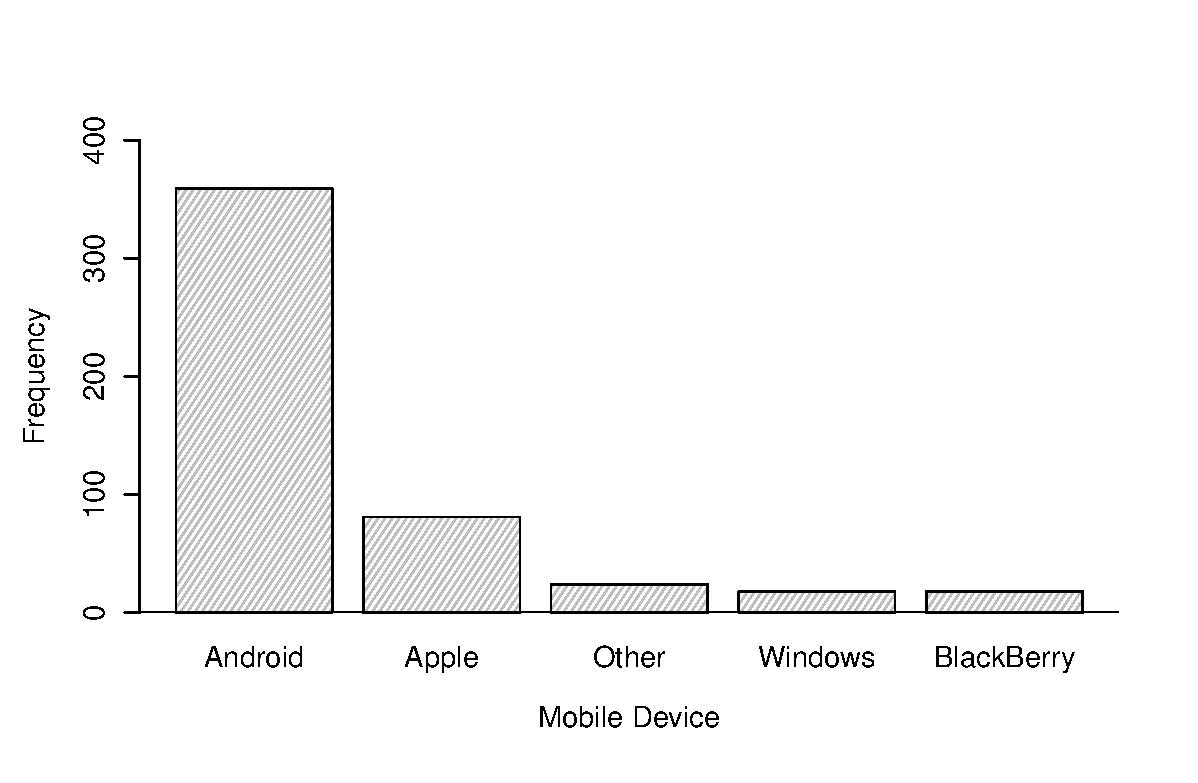
\includegraphics[width=0.9\textwidth, trim = 0.0cm 0.5cm 0.3cm 1.5cm, clip]{Bar2012}
\end{tabular}
\item[g)] Android now dominates the market.
\end{enumerate}
\end{minipage}
\end{minipage}}\vspace{0.03\textwidth}

\framebox[1.02\textwidth]{
\begin{minipage}[t]{0.98\textwidth}
\begin{minipage}[t]{0.47\textwidth}
\subsection*{Question 5}
It is usually helpful to rearrange the data:\\
\begin{small}
\begin{tabular}{|cccccccccc|}
\hline
0.1 & 0.2 & 0.2 & 0.4 & 0.7 & 0.7 & 0.9 & 1.0 & 1.0 & 1.4 \\
1.5 & 1.6 & 2.2 & 2.3 & 3.0 & 3.0 & 3.3 & 3.4 & 4.2 & 5.4 \\
5.6 & 5.7 & 6.1 & 12.9 & 14.3 &&&&& \\
\hline
\end{tabular}
\end{small}
\begin{enumerate}[a)]
\item $n = 25$. $\bar x = \frac{\sum x_i}{n} = \frac{81.1}{25}=3.244$ hours.
\item $\text{width} = \frac{\max(x)-\min(x)}{\text{\# of classes}} = \frac{14.3-0.1}{5}=\frac{14.2}{5}=2.84.$\\[0.2cm]
    Always round up the width $\Rightarrow$ width = 3.
\end{enumerate}
\end{minipage}\hspace{0.055\textwidth}
\begin{minipage}[t]{0.47\textwidth}
    Starting at 0 $\Rightarrow$ 0 - 3, 3 - 6, 6 - 9, 9 - 12, 12 - 15. \\[0.4cm]
    Classes: 0 - 2.9, 3 - 5.9, 6 - 8.9, 9 - 11.9, \\12 - 14.9. \\[2cm]
    (continued on next page)
\end{minipage}
\end{minipage}}


\framebox[1.02\textwidth]{
\begin{minipage}[t]{0.98\textwidth}
\begin{minipage}[t]{0.47\textwidth}
\subsection*{Question 5 - continued}
\begin{enumerate}
\item[b)]
\begin{tabular}{|c|r|r|}
\hline
&&\\[-0.4cm]
Class      & Freq. & R. Freq. \\
&&\\[-0.5cm]
\hline
&&\\[-0.4cm]
0 - 2.9   &   14     & $\tfrac{14}{25} = 0.56$ \\[0.2cm]
3 - 5.9   &    8     & $\tfrac{8}{25} = 0.32$ \\[0.2cm]
6 - 8.9   &    1     & $\tfrac{1}{25} = 0.04$ \\[0.2cm]
9 - 11.9  &    0     & $\tfrac{0}{25} = 0.00$ \\[0.2cm]
12 - 14.9 &    2     & $\tfrac{2}{25} = 0.08$ \\[0.2cm]
\hline
&&\\[-0.4cm]
\multicolumn{1}{|r|}{Total:} & $n = 25$ & $\tfrac{25}{25} = 1.00$ \\[0.1cm]
\hline
\end{tabular}
\item[c)] Relative frequencies in table above.
\item[d)] $\hat p_{(> 6 \text{ hrs})} = 0.04 + 0.00 + 0.08 = 0.12.$
\item[e)] The true proportion is called a \emph{parameter}.\newline Value: $p_{(> 6 \text{ hrs})} =$ unknown.
\end{enumerate}
\end{minipage}\hspace{0.055\textwidth}
\begin{minipage}[t]{0.47\textwidth}
\phantom{\qquad}
\begin{enumerate}
\item[f)]
\begin{tabular}{c}
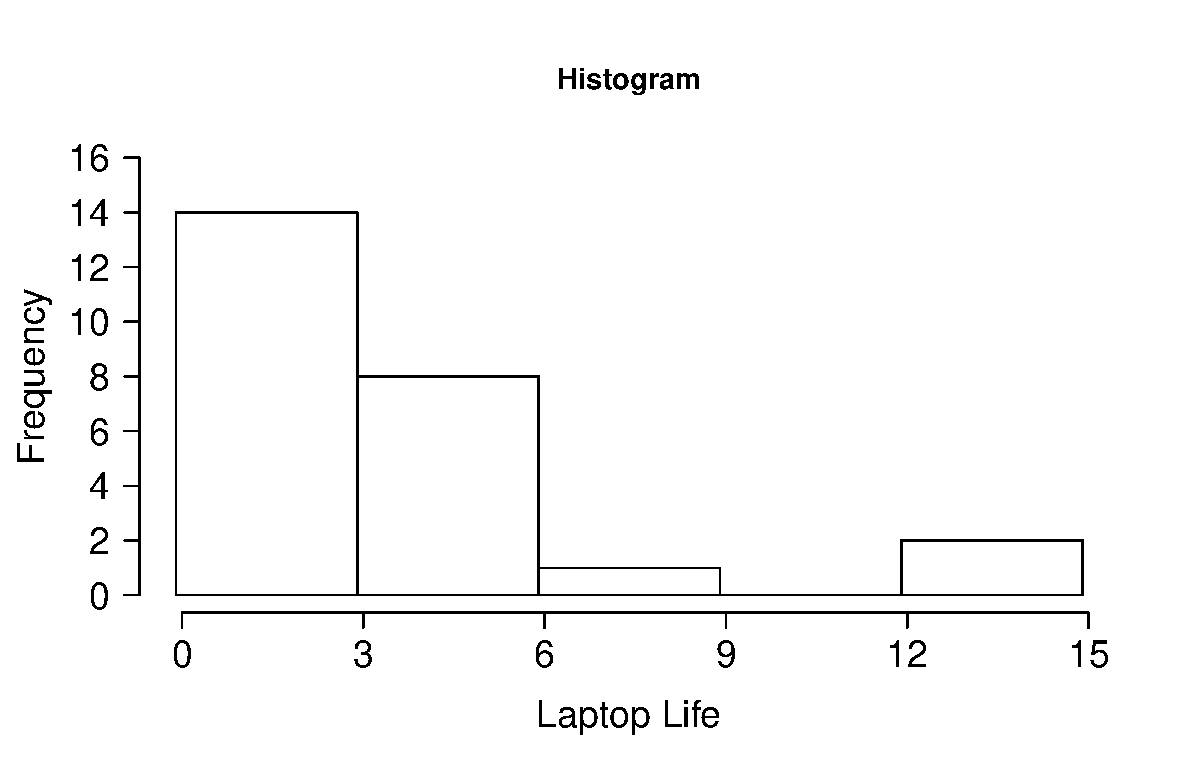
\includegraphics[width=0.9\textwidth, trim = 0.0cm 0.0cm 0.3cm 1.5cm, clip]{LaptopHist}
\end{tabular}
The data is skewed to the right.
\end{enumerate}
\end{minipage}
\end{minipage}}






%\framebox[0.5\textwidth]{
%\begin{minipage}[t]{0.46\textwidth}
%\subsection*{Question 2}
%\begin{enumerate}[a)]
%\item \emph{All} resistors produced.
%\item The 1520 resistors tested.\\[-0.3cm]
%\item The \emph{true} proportion of faulty resistors. Symbol: $p$. Value: unknown (must be estimated).\\[-0.3cm]
%\end{enumerate}
%\rule{1\textwidth}{1pt}
%\subsection*{Question 2}
%\begin{enumerate}[a)]
%\item \emph{All} resistors produced.
%\item The 1520 resistors tested.\\[-0.3cm]
%\item The \emph{true} proportion of faulty resistors. Symbol: $p$. Value: unknown (must be estimated).\\[-0.3cm]
%\end{enumerate}
%\end{minipage}}\vspace{0.03\textwidth}


\end{document} 